\clearpage
\section{Quantum Key Distribution Without Basis Switching}

\begin{refsection}

\begin{tcolorbox}	
\begin{tabular}{p{2.75cm} p{0.2cm} p{10.5cm}} 	
\textbf{Student Name}  &:&  Goncalo Nunes (2018/05/20- )\\
\textbf{Goal}          &:& Provide practical evidence of the employability of a coherent state quantum key distribution protocol based on simultaneous quadrature measurements.\\
\textbf{Directory}              &:& sdf/qkd\_with\_cv\_without\_base\_switching
\end{tabular}
\end{tcolorbox}Quantum key distribution (QKD) is a method to generate a cryptographic key between two distant parties, Alice and Bob, based on transmission of quantum states. After said transmission and respective measurement, Alice and Bob can then exchange classical messages through an insecure channel and, using the keys generated, perform post-processing to recover the messages.\\ 
In the first quantum key distribution schemes, single photons acted as information carriers (discrete variable regime). The practical implementation of said schemes was limited by the single photon generation and detection techniques. Hence the current interest in continuous variable (CV) quantum cryptography, which allows for higher key rates. The security of a CV-QKD relies on randomly switching the measurement basis (quadratures). In practice this implies a change of phase of a local oscillator beam which is difficult to achieve and constitutes a serious technical difficulty for the implementation of this type of cryptosystem, compromising its bandwidth.\\
Hence the pertinence of a QKD scheme that doesn't require for the change in measurement basis. Such protocol was analyzed in \cite{Weedbrook2004} and is called the simultaneous quadrature measurement or SQM Protocol, where both bases are measured simultaneously through double homodyne detection. It utilizes the quantum channel more effectively and achieves both higher secret key rates and bandwidths compared to orthodox CV-QKD protocols.
\subsection{Experimental Overview}
	\begin{figure}[H]
	\centering
	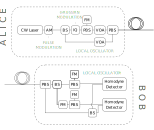
\includegraphics[width=0.8\textwidth,height=7cm]{./sdf/qkd_with_cv_without_base_switching/figures/setup.png}
	\caption{Experimental configuration of a continuous variable quantum key distribution. CW Laser, continuous wave laser; PBS, polarizing beam splitter; AM, amplitude modulator; PM, phase modulator; IQ, IQ modulator; BS, beam splitter; PBS, polarization beam splitter; VOA, variable optical attenuator.\label{fig:qkdwbs setup}}
\end{figure}

The scheme is similar to an ordinary continuous variable coherent state quantum cryptography protocol. To begin with, Alice produces a coherent state pulse with a continuous-wave laser (CW Laser) in combination with an amplitude modulator (AM). Using a beam splitter (BS), the pulse is then divided into two portions with an intensity ratio 1:99. The weak portion is modulated in phase and amplitude, changing the quadratures $\hat{X}^-$ and $\hat{X}^+$, respectively. This is achieved through the usage of an IQ modulator. The modulated signal's polarization is shifted 90 degrees using a Faraday mirror for future combination with a reference signal. Before, though, the variance is adjusted by tuning a variable optical attenuator (VOA). Meanwhile, the strong pulse is attenuated by a VOA to an optimal intensity. This signal acts as a reference, namely local oscillator, and together with the modulated signal constitutes the polarization-multiplex signal to be sent to Bob mixed with polarization beam splitter (PBS). The multiplexed signal is sent through a quantum channel, an optical fiber, to Bob.\\ At Bob's side the signal is demultiplex using again a PBS, splitting the modulated state and the reference. The reference signal is split using a 50:50 BS. Using a phase modulator (PM), part of the split local oscillator's phase is shifted $\pi/2$ for the measurement of $\hat{X}^+$ and another one is left unchanged for $\hat{X}^-$. The quadratures are measured through the comparison of the modulated signal with the local oscillator, using two homodyne detectors.
  
%\begin{figure}[h]
%\centering
%\includegraphics[width=.4\linewidth]{./sdf/bpsk_system/figures/bpskconstellation.jpg}
%\caption{BPSK symbol constellation.}
%\label{fig:BPSKConst}
%\end{figure}

% bibliographic references for the section ----------------------------
\clearpage
\printbibliography[heading=subbibliography]
\end{refsection}
\addcontentsline{toc}{subsection}{Bibliography}
\cleardoublepage
% --------------------------------------------------------------------- 